\documentclass[notes,professionalfont,11pt,usenames,dvipsnames]{beamer}

\usepackage{pxfonts}
\usepackage{eulervm}

\usepackage{pgf,pgfarrows,pgfnodes,pgfautomata,pgfheaps,pgfshade}
\usepackage{tikz}
\usetikzlibrary{plothandlers,plotmarks,arrows,automata}
\usepackage{amsmath,amssymb}
\usepackage{colortbl}
\usepackage[latin1]{inputenc}
\usepackage{mathrsfs}
\renewcommand{\mathcal}{\mathscr}
\usepackage{enumerate}

\newcommand\independent{\protect\mathpalette{\protect\independenT}{\perp}}
\def\independenT#1#2{\mathrel{\rlap{$#1#2$}\mkern2mu{#1#2}}}

\newcommand\smpl{\mathcal{D}_n}
\newcommand\dsplnt{\displaystyle\int}
\newcommand{\disp}{\displaystyle}
\newcommand{\ds}{\displaystyle}
\newcommand{\vs}{\bigskip}
\newcommand{\esp}{\mathbb E}
\newcommand{\prob}{\mathbb P}
\newcommand{\ee}{\mathrm e}
\newcommand{\ii}{\mathrm i}
\newcommand{\dd}{\text{d}}
\newcommand{\Int}{\mathrm{int}\,}
\newcommand{\Cl}{\mathrm{adh}\,}
\newcommand{\Supp}{\operatorname{Supp}}
\newcommand{\Card}{\operatorname{Card}}
\newcommand{\Var}{\operatorname{Var}}
\newcommand{\Ave}{\operatorname{Ave}}
\renewcommand{\mathcal}{\mathscr}

\newcommand{\logit}{\operatorname{logit}}
\renewcommand{\epsilon}{\varepsilon}
\newcommand{\eps}{\varepsilon}
\newfont{\manfnt}{manfnt}
\newcommand{\danger}{{\manfnt\symbol{'177}}}
\newcommand{\mdanger}{\marginpar[\hfill\danger]{\danger\hfill}}
\newcommand{\new}{{\manfnt\symbol{30}}}
\newcommand{\mnew}{\marginpar[\hfill\new]{\hfill\new}}
\renewcommand{\P}{\mathbb{P}}
\newcommand{\E}{\mathbb{E}}
\newcommand{\V}{\mathbb{V}}
\newcommand{\tbrown}[1]{\textcolor{brown}{#1}}
\DeclareTextFontCommand{\hershey}{\fontfamily{hscs}\selectfont}
\newcommand{\tb}{\color{brown}}

\usetheme{Boadilla}
\usecolortheme{rose}

\newcommand\justify{\rightskip0pt \leftskip0pt}

%\usetheme{Goettingen}

\newenvironment{slide}
{\begin{frame}[environment=slide]
\frametitle{\insertsection \\ \insertsubsection}\justify\setlength{\parskip}{0.5cm}\vspace{-1cm}}
{\end{frame}}


\setbeamersize{text margin left=1cm}
\setbeamersize{text margin right=1cm}

%\setbeamersize{sidebar width left=1cm}
%\setbeamersize{sidebar width right=1cm}

\makeatletter
\newcommand{\setnextsection}[1]{%
  \setcounter{section}{\numexpr#1-1\relax}%
  \beamer@tocsectionnumber=\numexpr#1-1\relax\space}
\makeatother

\setbeamertemplate{itemize items}[triangle]
\setbeamercolor{itemize item}{fg=brown}
\setbeamertemplate{enumerate items}[circle]
\setbeamercolor{item projected}{bg=brown}
\setbeamercolor{block title}{fg=brown!100, bg=gray!20}
\setbeamercolor{block body}{bg=gray!10}

\title[Bayesian parameter inference]{Bayesian parameter inference}
\author[Jean-Michel Marin]{Jean-Michel Marin}

\institute[IMAG]{University of Montpellier \\
Faculty of Sciences}

\date[HAX918X]{HAX918X / 2024-2025}

\begin{document}

\frame{\titlepage}

\frame{\tableofcontents} 

\section{The Bayesian paradigm}

\begin{slide}

The interpretation of probability depends on different epistemological frameworks, and there are several philosophical approaches to understanding what probability means

long-run frequency of events /
degree of belief in a hypothesis

\textbf{Subjectivism}

Harold Jeffreys (1891-1989)

Frank Plumpton Ramsey (1903-1930)

Bruno de Finetti (1906-1985)

Leonard Jimmie Savage (1921-1971)


\end{slide}

\begin{slide}

Subjectivism in probability refers to the interpretation that probabilities represent personal beliefs or degrees of certainty about uncertain events

{\color{red} \bf It contrasts with objective interpretations, viewing probability as a subjective measure based on individual judgment rather than frequency or inherent properties}

Subjectivists argue that probabilities can vary between individuals based on their information and perspective 

Bayesian probability, which updates beliefs as new information becomes available, is a key framework in this approach

\end{slide}

\begin{slide}

R.A. Fisher (1890-1962) and Harold Jeffreys (1891-1989) 

The Jeffreys-Fisher conflict is a most important episode in the recent history of scientific ideas. Both were themselves eminent mathematical scientists: Fisher a statistician and geneticist, Jeffreys a geophysicist 

The controversy between R.A. Fisher and Harold Jeffreys was centered around differing interpretations of probability and statistical inference 

\end{slide}

\begin{slide}

{\color{red} \bf Interpretation of Probability}

Fisher (Frequentist Approach): Fisher viewed probability as a long-run frequency of events. According to the frequentist interpretation, probability is defined through repeated experiments: the probability of an event is the proportion of times it occurs in a large number of trials
   
\vs Jeffreys (Bayesian Approach): Jeffreys, on the other hand, embraced a subjective interpretation of probability. He believed that probability measures the degree of belief in a hypothesis, which can be updated with new evidence

\end{slide}

\begin{slide}

{\color{red} \bf Hypothesis Testing}

Fisher developed the method of significance testing, focusing on p-values as a measure of evidence against the null hypothesis. He believed that if the p-value was below a threshold (often 0.05), the null hypothesis could be rejected. He did not require an explicit alternative hypothesis, focusing more on the ability to reject or retain the null hypothesis

Jeffreys was critical of p-values and focused on Bayes factors, which compare the likelihood of the data under two competing hypotheses (the null and the alternative). Bayesian hypothesis testing incorporates prior information and gives a more direct comparison between the two hypotheses

\end{slide}

\begin{slide}

{\color{red} \bf Use of Prior Information}

Fisher was critical of using prior probabilities, especially when they were subjective or arbitrary. He believed that statistical inference should be based on the data at hand without needing prior beliefs

\vs Jeffreys, in contrast, argued that it was natural and necessary to incorporate prior information into statistical analysis. His approach, known as Bayesian inference, updates prior beliefs with data to produce a posterior probability, using Bayes' theorem


\end{slide}

\begin{slide}

{\color{red} \bf Likelihood Principle}

Fisher strongly promoted the likelihood principle, arguing that the likelihood function (the probability of observing the data given different parameter values) was key in statistical inference. He introduced the idea of maximum likelihood estimation (MLE) to find the parameter values that maximize the likelihood of the observed data

\vs Jeffreys agreed that the likelihood function is important but argued that it should be integrated with prior probabilities to produce posterior probabilities for parameters, a key feature of Baye\-sian statistics

\end{slide}

\begin{slide}

{\color{red} \bf Core of the Controversy}

Fisher's frequentist approach was based on using data to make conclusions about hypotheses without reference to prior beliefs

Jeffreys' Bayesian approach involved incorporating prior knowledge and using Bayes' theorem to update the probability of a hypothesis given new data

{\color{red} Both approaches have strengths and limitations, and modern statistics has, in many cases, integrated elements of both Fisherian and Bayesian thinking}

\end{slide}

\begin{slide}

Fisher's frequentist methods have become standard in many scientific disciplines, especially in hypothesis testing and estimation techniques

Jeffreys' Bayesian ideas gained more prominence in the latter half of the 20th century, especially with the rise of computational power, allowing for more complex Bayesian analyses

\end{slide}

\begin{slide}

\begin{center} 
\bf Bayes theorem = Inversion of probabilities 
\end{center}

If $A$ and $B$ are events such that $\P(B)\neq 0$,
$$
\P(A|B)=\frac{\P(A\cap B)}{\P(B)}=\frac{\P(B|A)\P(A)}{\P(B)}
=
$$
$$
\frac{\P(B|A)\P(A)}{\P(A)\P(B|A)+\P(\bar A)\P(B|\bar A)}
$$

\end{slide}


\begin{slide}

Given an iid sample $\mathcal{D}_n=(x_1,\ldots,x_n)$
from a density $f(x|\theta)$, depending upon an unknown parameter
$\theta\in\Theta$, the associated likelihood function is
$$
f(\mathcal{D}_n|\theta) = \prod_{i=1}^n f(x_i|\theta) = \ell(\theta|\mathcal{D}_n)
$$

\end{slide}

\begin{slide}

When $\mathcal{D}_n$ is a normal $\mathcal{N}(\mu,\sigma^2)$ sample of size $n$ and
$\theta=(\mu,\sigma^2)$, we get
\begin{align*}
\ell(\theta|\mathcal{D}_n) &= \prod_{i=1}^n \exp\{ -(x_i-\mu)^2/2\sigma^2 \} / \sqrt{2\pi}\sigma \\
&\propto \exp\left\{ -\sum_{i=1} (x_i-\mu)^2/2\sigma^2 \right\}/\sigma^n \\
&\propto \exp\left\{ - \left(n \mu^2 -2n\bar x\mu + \sum_{i=1} x_i^2 \right)\big/ 2\sigma^2 \right\}/\sigma^n \\
&\propto \exp\left\{ - \left[n (\mu -\bar x)^2 + s^2 \right]\big/ 2\sigma^2 \right\}/\sigma^n,
\end{align*}
$\bar x$ denotes the empirical mean and $s^2=\sum_{i=1}^n  (x_i-\bar x)^2$

\end{slide}

\begin{slide}

{\color{red}\bf In the Bayesian approach $\theta$ is considered as a random variable}

In some sense, the likelihood function
is transformed into a {\em posterior} distribution, which is a 
valid probability distribution on $\Theta$ 
$$
\pi(\theta|\mathcal{D}_n) = \frac{\ell(\theta|\mathcal{D}_n)\pi(\theta)}{
\int\,\ell(\theta|\mathcal{D}_n)\pi(\theta)\,\hbox{d}\theta}
$$

$\pi(\theta)$ is called the {\em prior} distribution and it has to be chosen 
to start the analysis

\end{slide}

\begin{slide}

The posterior density is a probability density on the parameter, which does not mean the parameter $\theta$ 
need be a genuine random variable

{\color{red}\bf This density is used as an inferential tool,
not as a truthful representation}

\end{slide}

\begin{slide}

Two motivations:
\begin{itemize}
\item the prior distribution summarizes the {\em 
prior information} on $\theta$. However, the choice of $\pi(\theta)$
is often decided on practical grounds rather than strong
subjective beliefs
\item the Bayesian approach provides a fully probabilistic 
framework for the inferential analysis,
with respect to a reference measure $\pi(\theta)$
\end{itemize}

\end{slide}

\begin{slide}

Suppose $\mathcal{D}_n$ is a normal $\mathcal{N}(\mu,\sigma^2)$ sample of size $n$

When $\sigma^2$ is known, if $\mu\sim\mathcal{N}\left(0,\sigma^{2} \right)$, 
then
\begin{align*}
\pi(\mu|\mathcal{D}_n) &\propto \pi(\mu)\,f(\mathcal{D}_n|\mu)\\
&\propto \pi(\mu)\,\ell(\mu|\mathcal{D}_n)\\
&\propto \exp\{-\mu^2/2\sigma^2\}\,\exp\left\{-n(\bar x-\mu)^2/2\sigma^2 \right\}\\
&\propto \exp\left\{ -(n+1)\mu^2/2\sigma^2 + 2n\mu\bar x/2\sigma^2 \right\}\\
&\propto \exp\left\{ -(n+1)[\mu-n\bar x/(n+1)]^2/2\sigma^2 \right\}
\end{align*}


\centerline{\color{red}\fbox{
$
\mu|\mathcal{D}_n\sim\mathcal{N}\left(n\bar x/(n+1),\sigma^2/(n+1)\right)
$
}}

\end{slide}

\begin{slide}

When $\sigma^2$ is unknown, $\theta=(\mu,\sigma^2)$, if 
$\mu|\sigma^2\sim \mathcal{N}\left(0,\sigma^{2}\right)$ and $\sigma^2\sim\mathcal{IG}(1,1)$, then
$\pi((\mu,\sigma^2)|\mathcal{D}_n)\propto \pi(\sigma^2)\times\pi(\mu|\sigma^2)\times f(\mathcal{D}_n|\mu,\sigma^2)$
$$
\propto (\sigma^{-2})^{1/2+2}\exp\left\{-(\mu^2 + 2)/2\sigma^2\right\}\mathbf{1}_{\sigma^2>0}
$$
$$
(\sigma^{-2})^{n/2}\exp\left\{-\left(n(\mu-\overline{x})^2 + s^2 \right)/2\sigma^2\right\}
$$


\centerline{\color{red}\fbox{
$\ds \mu|\mathcal{D}_n,\sigma^2\sim \mathcal{N}\left(\frac{n\bar x}{n+1},\frac{\sigma^2}{n+1}\right)$}}

\vs \centerline{\color{red}\fbox{
$\ds \sigma^2|\mathcal{D}_n\sim \mathcal{IG}\left(\left\{1+\frac{n}{2}\right\},\left\{1+\frac{s^2}{2}+\frac{n\bar x}{2(n+1)}\right\}\right)$}}

\end{slide}

\begin{slide}

Variability in $\sigma^2$ induces more variability in $\mu$, the marginal 
posterior in $\mu$ being then a Student's $t$ distribution


\vs \centerline{\color{red}\fbox{
$\ds \mu|\mathcal{D}_n \sim \mathcal{T}\left(n+2,\frac{n\bar x}{n+1},\frac{2+s^2+(n\bar x)/(n+1)}{(n+1)(n+2)}\right)$
}}

\end{slide}

\section{Bayesian estimates}

\begin{slide}

For a given loss function $L\left(\theta,\hat\theta(\mathcal{D}_n)\right)$,
we deduce a Bayesian estimate by minimizing the posterior expected loss:
$$
\E^\pi_{\theta|\mathcal{D}_n}\left(L\left(\theta,\hat\theta(\mathcal{D}_n)\right)\right)
$$


{\bf \color{red} To minimize the posterior expected loss 
is equivalent to minimize the Bayes risk, 
the frequentist risk integrated over the prior distribution
}

\end{slide}

\begin{slide}

For instance, for the $L_2$ loss function,
the corresponding Bayes optimum is the expected value of $\theta$
under the posterior distribution,
$$
\hat\theta(\mathcal{D}_n) = \int \theta \,\pi(\theta|\mathcal{D}_n)\,\hbox{d}\theta
                          = \frac{\int \theta\,\ell(\theta|\mathcal{D}_n)\,\pi(\theta)\,\hbox{d}\theta}
                           {\int \ell(\theta|\mathcal{D}_n)\,\pi(\theta)\,\hbox{d}\theta}
$$

\end{slide}

\begin{slide}
\begin{minipage}{\linewidth}

When no specific penalty criterion is available, the posterior expectation is often used
as a default estimator, although alternatives are also available. For 
instance, the {\em maximum a posteriori estimator} (MAP) is defined as
$$
\hat\theta(\mathcal{D}_n) \in \text{argmax}_\theta \quad\pi(\theta|\mathcal{D}_n)
$$


{\bf \color{red} Similarity of with the maximum likelihood estimator: the influence of the prior
distribution $\pi(\theta)$ on the estimate progressively disappears as the number
of observations $n$ increases}

\end{minipage}
\end{slide}

\section{Conjugate prior}

\begin{slide}

The selection of the prior distribution is an important issue in
Bayesian statistics


When prior information is available about the
data or the model, it can be used in building the prior 


In many situations, however, the selection of the prior distribution is quite delicate


{\bf \color{red} Since the choice of the prior distribution has a considerable influence on
the resulting inference, this inferential step must be conducted with the utmost care}

\end{slide}

\begin{slide}

{\bf Conjugate priors are such that the prior and posterior densities belong to the same parametric family}


An advantage when using a conjugate prior, is that one has to select only
a few parameters to determine the prior distribution 


But the information known a priori may be either insufficient or 
incompatible with the structure imposed by conjugacy

\end{slide}

\begin{slide}
\begin{minipage}{\linewidth}

Justifications
\begin{itemize}
\item Device of virtual past observations
\item First approximations to adequate priors, backed up by robustness
analysis
\item But mostly... tractability and simplicity
\end{itemize}

\end{minipage}
\end{slide}

\begin{slide}
\begin{minipage}{\linewidth}

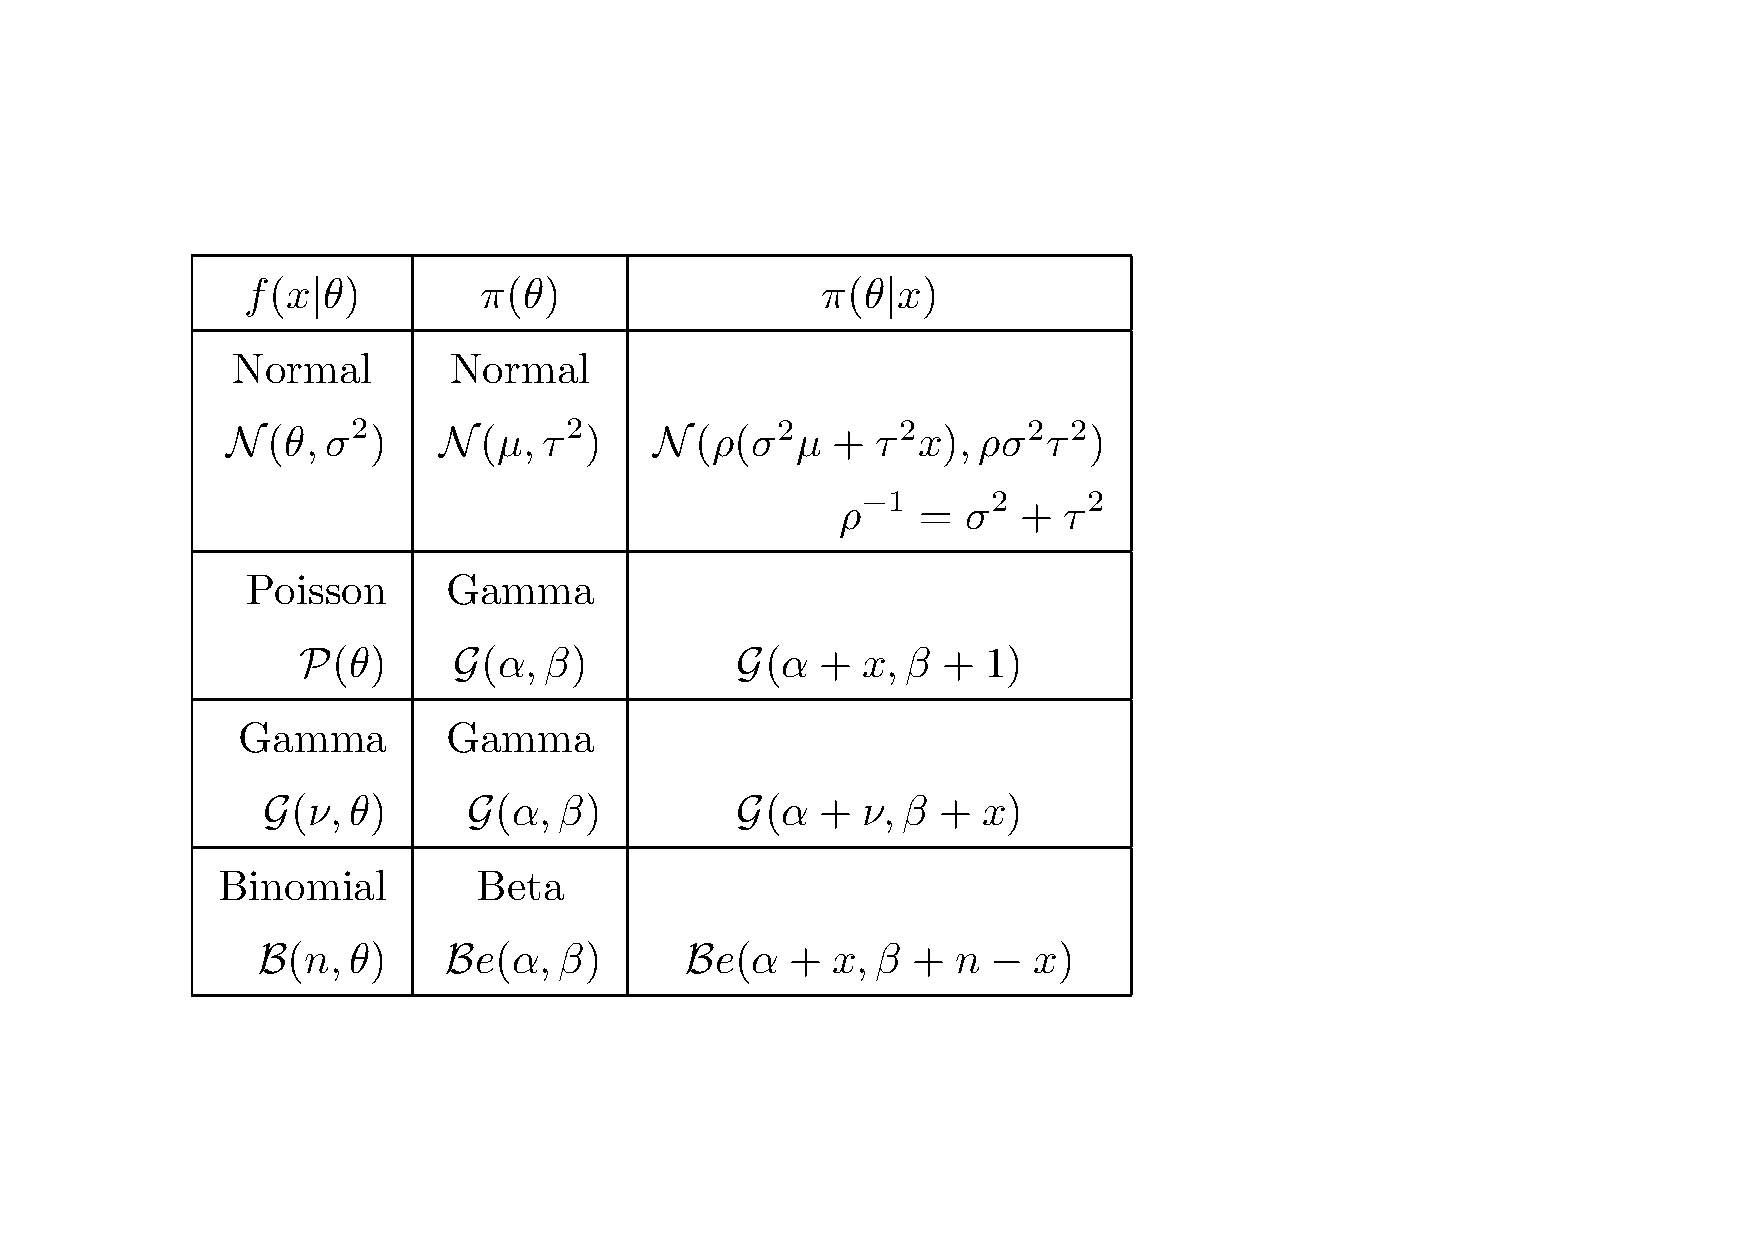
\includegraphics[scale=0.45]{add4.pdf}

\end{minipage}
\end{slide}

\begin{slide}
\begin{minipage}{\linewidth}

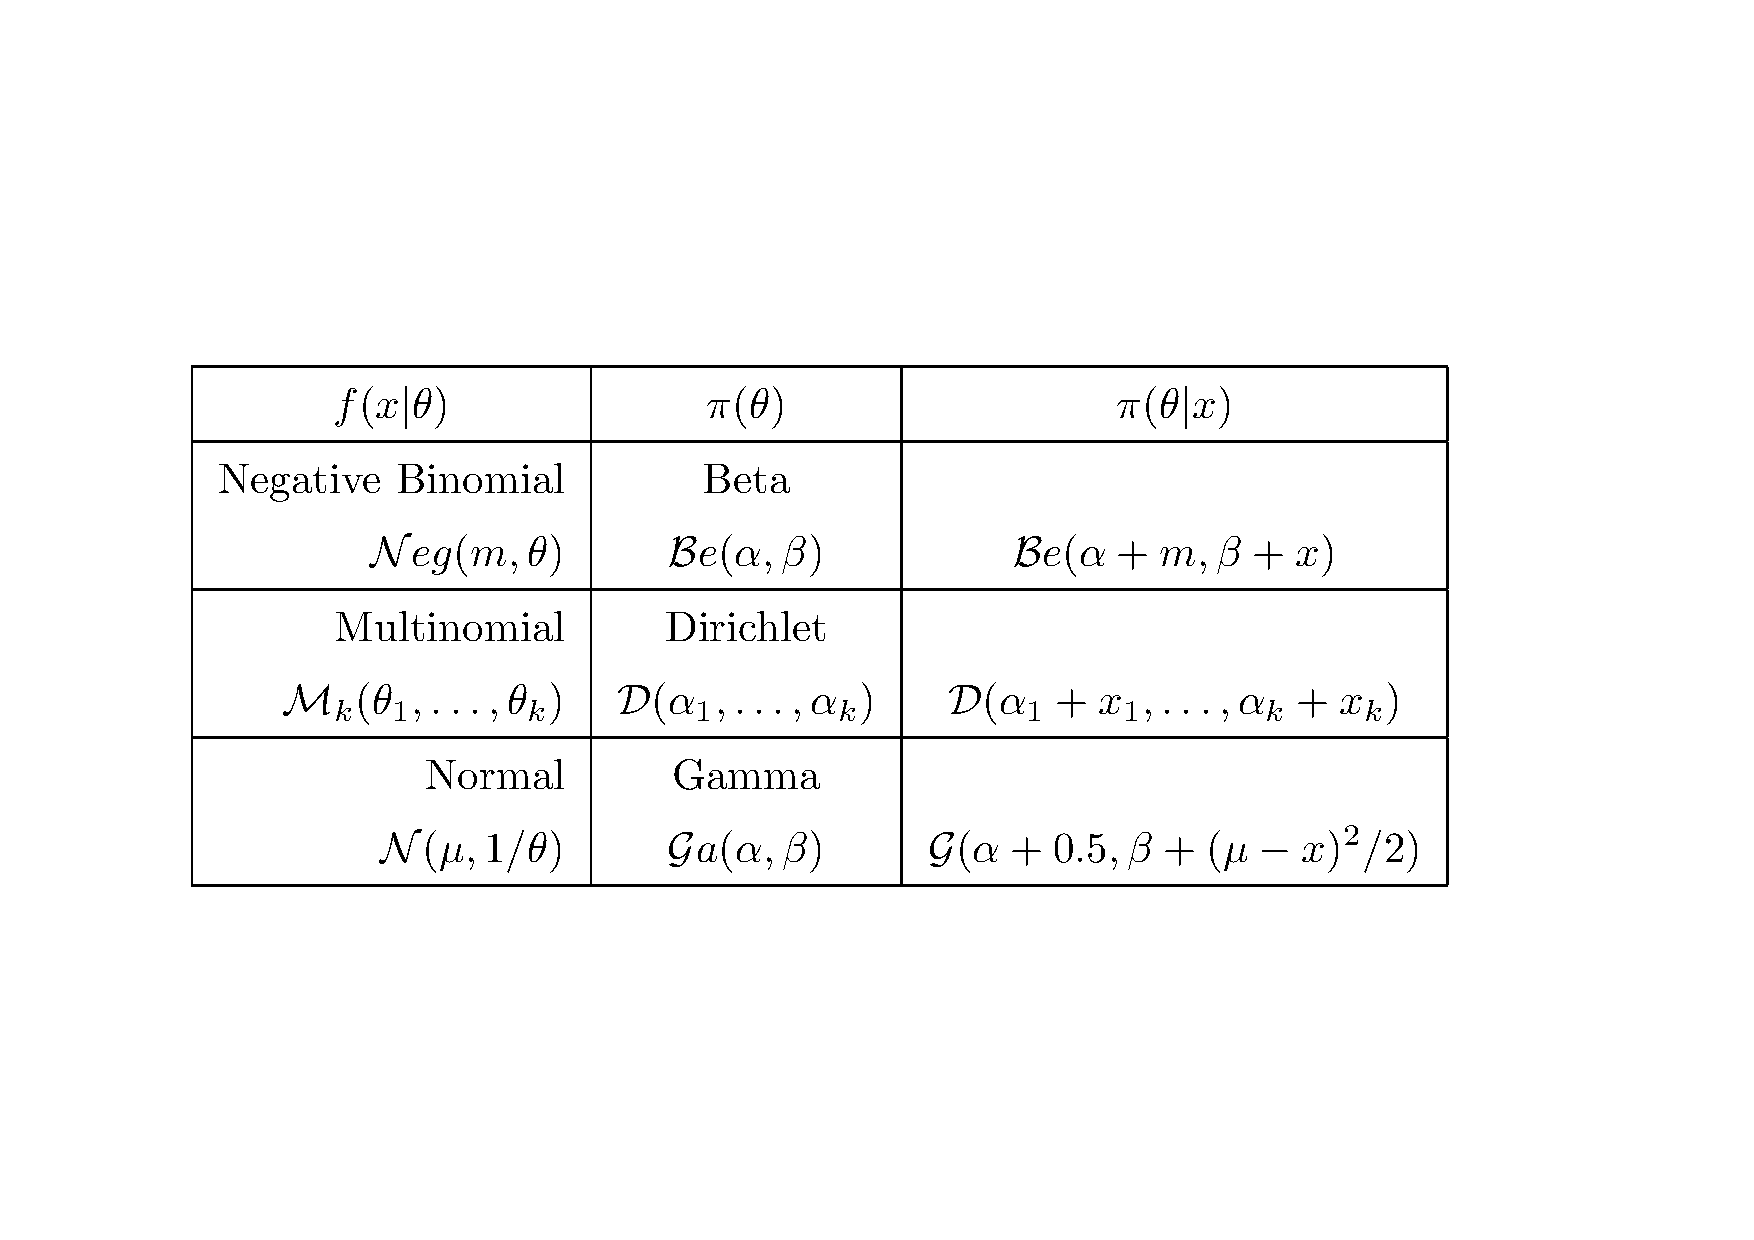
\includegraphics[scale=0.45]{add5.pdf}

\end{minipage}
\end{slide}

\section{Noninformative prior}

\begin{slide}

Conjugate priors are nice to work with, 
but require hyperparameters's determination


One can opt for a completely different perspective 
and rely on so-called {\em noninformative} priors that aim at attenuating the impact 
of the prior on the resulting inference


These priors are fundamentally defined as coherent extensions of the uniform distribution

\end{slide}

\begin{slide}

For unbounded parameter spaces, the densities of noninformative
priors actually may fail to integrate to a finite number and they are defined
instead as positive measures


{\bf\color{red} Generalized Bayesian estimators with improper \\ prior distributions}

\end{slide}

\begin{slide}

{\bf Location models} $x|\theta \sim f(x-\theta)$
are usually associated with flat priors $\pi(\theta)\propto 1$


{\bf Scale models} $x|\theta \sim \frac{1}{\theta}\,f\left(\frac{x}{\theta}\right)$
are usually associated with the log-transform of a flat prior, that is,
$\pi(\theta) \propto 1/\theta\times \mathbf{1}_{\theta>0}$

\end{slide}

\section{Jeffreys prior}

\begin{slide}

In a more general setting, the noninformative prior favored by most Ba\-ye\-si\-ans is
the so-called {\bf Jeffreys prior} 
which is related to the Fisher information matrix 
$$
I_x^F(\theta) = -\mathbb{E}\left(\dfrac{\partial^2 \log f(x|\theta) }{ (\partial \theta)^2}\right)
$$
by
$$
\pi^J(\theta) \propto \sqrt{\left| I_x^F(\theta) \right]}\times \mathbf{1}_{\theta\in\Theta}\,,
$$
where $|I|$ denotes the determinant of the matrix $I$

\end{slide}

\begin{slide}

Suppose $\mathcal{D}_n$ is a normal $\mathcal{N}(\mu,\sigma^2)$ sample of size $n$
and $\theta=(\mu,\sigma^2)$


The Fisher information matrix leads to the Jeffreys prior
$$
\pi^J(\mu,\sigma^2) \propto 1/\{\left(\sigma^2\right)\}^{3/2}\mathbf{1}_{\sigma^2>0}
$$


\vs \centerline{\color{red}\fbox{
$
\mu|\sigma^2,\mathcal{D}_n\sim\mathcal{N}\left(\bar x,\sigma^2/n\right)
$
}}

\vs \centerline{\color{red}\fbox{
$
\sigma^2|\mathcal{D}_n\sim\mathcal{IG}\left(n/2,s^2/2 \right)
$
}}

\vs \centerline{\color{red}\fbox{
$
\mu|\mathcal{D}_n \sim \mathcal{T}\left(n,\bar x,s^2/n\right)
$
}}

\end{slide}

\section{Bayesian Credible Intervals}

\begin{slide}

Since the Bayesian approach processes $\theta$ as a random variable, a natural definition
of a confidence region on $\theta$ is to determine $C(\mathcal{D}_n)$ such that
$$  
\pi(\theta\in C(\mathcal{D}_n) | \mathcal{D}_n) = 1-\alpha
$$
where $\alpha$ is a predetermined level


{\bf\color{red} The integration is done over the parameter space, rather than over the observation space}


The quantity $1-\alpha$ thus corresponds to the probability that a random $\theta$ belongs to this set
$C(\mathcal{D}_n)$, rather than to the probability that the random set contains
the true value of $\theta$

\end{slide}

\begin{slide}

Given this drift in the interpretation of a
confidence set is called a {\em credible set} by Bayesians.

 A standard credible set corresponds to the values of $\theta$ with the
highest posterior values,
$$
C(\mathcal{D}_n)=\left\{\theta;\,\pi(\theta|\mathcal{D}_n) \ge k_\alpha \right\}
$$
where $k_\alpha$ is determined by the coverage constraint


This region is called the {\bf Highest Posterior Density} (HPD) region

\end{slide}

\begin{slide}

Once again, suppose $\mathcal{D}_n$ is a normal $\mathcal{N}(\mu,\sigma^2)$ sample of size $n$
and $\theta=(\mu,\sigma^2)$

\vs \centerline{\color{red}\fbox{
$
\mu|\sigma^2,\mathcal{D}_n\sim\mathcal{N}\left(\bar x,\sigma^2/n\right)
$
}}

\vs \centerline{\color{red}\fbox{
$
\sigma^2|\mathcal{D}_n\sim\mathcal{IG}\left(n/2,s^2/2 \right)
$
}}

\vs \centerline{\color{red}\fbox{
$
\mu|\mathcal{D}_n \sim \mathcal{T}\left(n,\bar x,s^2/n\right)
$
}}


Therefore, the credible interval of probability $1-\alpha$ on $\mu$ is
$$
[\bar x-t_{1-\alpha/2,n}\sqrt{s^2/n},\bar x+t_{1-\alpha/2,n}\sqrt{s^2/n}]
$$

\label{lastslide}

\end{slide}

\end{document}